%----------------------------------------------------------------------------------------
%    PACKAGES AND THEMES
%----------------------------------------------------------------------------------------

\documentclass[aspectratio=169,xcolor=dvipsnames]{beamer}
\usetheme{SimpleDarkBlue}


\usepackage{cancel}
\usepackage{hyperref}
\usepackage{graphicx} % Allows including images
\usepackage{booktabs} % Allows the use of \toprule, \midrule and \bottomrule in tables
\usepackage{braket}

%----------------------------------------------------------------------------------------
%    TITLE PAGE
%----------------------------------------------------------------------------------------

\title{Hamiltonian Simulation}
\subtitle{Quantum Computing}

\author{Álvaro Sánchez-Paniagua, Ana Vargas, Gonzalo Martínez de Sola, Iñigo Iriondo, Miguel Laredo}

\institute
{
    Based on the notes from Ashley Montaro % Your institution for the title page
}
\date{\today} % Date, can be changed to a custom date

%----------------------------------------------------------------------------------------
%    PRESENTATION SLIDES
%----------------------------------------------------------------------------------------

\begin{document}

\begin{frame}
    % Print the title page as the first slide
    \titlepage
\end{frame}

\begin{frame}{Motivation}
\end{frame}


%\begin{frame}{Overview}
    % Throughout your presentation, if you choose to use \section{} and \subsection{} commands, these will automatically be printed on this slide as an overview of your presentation
%    \tableofcontents
%\end{frame}





%%%%%%%%%%%%%%%%%%%
% Ana
%%%%%%%%%%%%%%%%%%%

\section{Introduction}
\begin{frame}{Introduction: Hamiltonian \textcolor{lightgray}{Simulation}}
    \begin{block}{Hamiltonian}
        Hermitian operator acting on $n$ qubits which corresponds physically to a system made up of $n$ 2-level subsystems.
    \end{block}
    \begin{block}{Schrödinger’s equation}
        Time evolution of the state $|\psi\rangle$ of a quantum system:
        \begin{align*}
            i \hbar \frac{d}{dt}|\psi(t)\rangle = H(t)|\psi(t)\rangle
        \end{align*}
    \end{block}
\end{frame}

\begin{frame}{Introduction: \textcolor{lightgray}{Hamiltonian} Simulation}
    Solution of the Schrödinger’s equation (\textit{time-independent}):
    \begin{align*}
        |\psi(t)\rangle = e^{-iHt}|\psi(0)\rangle
    \end{align*}
    \begin{block}{Goal}
        To approximate the unitary operator:
        \begin{align*}
            U(t) =  e^{-iHt}
        \end{align*}
    \end{block}
    Approximation in the operator (spectral) norm:
    \begin{align*}
        ||A|| := \max_{|\psi\rangle \neq 0}\frac{||A|\psi\rangle||}{|||\psi\rangle||}.
    \end{align*}
    $\~{U}$ approximates $U$ within $\epsilon$ if
        \begin{align*}
            ||\~{U} - U|| < \epsilon
        \end{align*}
\end{frame}


%%%%%%%%%%%%%%%%%%%
% Alvaro
%%%%%%%%%%%%%%%%%%%

%------------------------------------------------
\section{Simulation of weighted sums of Pauli matrices}
%------------------------------------------------

\begin{frame}{Quantum Simulation of a Hamiltonian}

\textbf{Objective:} Efficiently simulate a Hamiltonian \( H \) using a quantum circuit. Specifically, approximate the time evolution operator:
\[
U = e^{-iHt}
\]
with a quantum circuit composed of a polynomial number of gates (\(\text{poly}(n)\)).

\medskip

\textbf{Focus:} We consider Hamiltonians acting on a Hilbert space of dimension \( 2^n \), i.e., matrices of size \( 2^n \times 2^n \).

\medskip

\textbf{Key Question:}  
How can a Hamiltonian, which has exponentially many parameters, be approximated by a quantum circuit that only contains polynomially many parameters (poly(\(n\)) gates)?

\end{frame}



\begin{frame}{Hamiltonians as Sums of Pauli Matrices}

\textbf{Motivation:}  
To efficiently simulate quantum systems, we leverage certain physical properties that allow for an efficient decomposition.

\medskip

\textbf{Pauli Decomposition of Hamiltonians:}  
We consider Hamiltonians expressed as sums of Pauli matrices acting on \( n \) qubits.

\medskip

\textbf{Notation:}  
For \( s \in \{I, X, Y, Z\}^n \), we define the matrix \( \sigma_s \) as the tensor product of the corresponding Pauli matrices:
\[
\sigma_s = s_1 \otimes s_2 \otimes \dots \otimes s_n.
\]
For example:
\[
\sigma_{ZX} = Z \otimes X.
\]

\end{frame}


\begin{frame}{Representation of Hamiltonians}

\textbf{Key Idea:} Any Hermitian \(2^n \times 2^n\) matrix can be decomposed as a sum of Pauli matrices like we previously said:
\[
H = \sum_{s \in \{I, X, Y, Z\}^n} \alpha_s\, \sigma_s
\]
where the coefficients \(\alpha_s\) are real numbers.

\bigskip

\textbf{Why is this useful and makes any sense?}
\begin{itemize}
    \item \textcolor{blue}{Pauli matrices form a basis} for all \(2^n \times 2^n\) Hermitian matrices.
    \item If only \textcolor{red}{a polynomial number of coefficients} are nonzero, then \(H\) can be simulated efficiently.
    \item This sparsity is not arbitrary—it corresponds to physical Hamiltonians with \textcolor{green}{local interactions}.
\end{itemize}

\end{frame}
% Add this to your preamble if needed:
% \usepackage{amsmath} 
% \usepackage{amssymb}

\begin{frame}{Step 1: The Pauli Matrices as a Basis}
\textbf{Pauli Matrices (for 1 qubit):}
\[
I = \begin{pmatrix} 1 & 0 \\ 0 & 1 \end{pmatrix}, \quad
X = \begin{pmatrix} 0 & 1 \\ 1 & 0 \end{pmatrix}, \quad
Y = \begin{pmatrix} 0 & -i \\ i & 0 \end{pmatrix}, \quad
Z = \begin{pmatrix} 1 & 0 \\ 0 & -1 \end{pmatrix}.
\]

\textbf{Generalized Pauli Basis (for \(n\) qubits):}
\[
\sigma_s = s_1 \otimes s_2 \otimes \cdots \otimes s_n, \quad s_i \in \{I, X, Y, Z\}
\]

\vspace{0.2cm}
\textbf{Goal:} Prove these matrices form an orthonormal basis for \(2^n \times 2^n\) Hermitian matrices.

\vspace{0.2cm}
\textbf{Key Steps:}
\begin{itemize}
    \item Show linear independence.
    \item Prove they span the entire space.
    \item Use the Hilbert-Schmidt inner product:
    \[
    \langle A, B \rangle = \frac{1}{2^n} \text{Tr}(A^\dagger B)
    \]
\end{itemize}

\vspace{0.2cm}
\textbf{Why the Trace?}
\begin{itemize}
    \item Measures "overlap" between matrices.
    \item Invariant under basis changes.
    \item Simplifies orthogonality proofs.
\end{itemize}
\end{frame}

% --- New Frame: Intuition Behind the Trace ---
\begin{frame}{Intuition: The Trace as a Similarity Check}
\small
\textbf{Analogy:} The trace \(\text{Tr}(A^\dagger B)\) acts like a "dot product" for matrices.

\vspace{0.2cm}
\textbf{Example (1 qubit):}
\[
\text{Tr}(X Z) = \text{Tr}\left(\begin{pmatrix} 0 & 1 \\ 1 & 0 \end{pmatrix}\begin{pmatrix} 1 & 0 \\ 0 & -1 \end{pmatrix}\right) = \text{Tr}\begin{pmatrix} 0 & -1 \\ 1 & 0 \end{pmatrix} = 0 + 0 = 0.
\]
\[
\text{Tr}(X X) = \text{Tr}(I) = 2.
\]

\vspace{0.2cm}
\textbf{Key Insight:}
\begin{itemize}
    \item Different Pauli matrices: \(\text{Tr}(S_i S_j) = 0\) (orthogonal).
    \item Same Pauli matrices: \(\text{Tr}(S_i S_j) = 2\).
\end{itemize}

\vspace{0.2cm}
\textbf{General Case:}
For \(S_i \neq S_j\), \(\text{Tr}(S_i S_j) = 0 \implies\) No overlap \(\implies\) Independent!
\end{frame}

% --- Step 2: Proving Orthogonality ---
\begin{frame}{Step 2: Proving Orthogonality}
\textbf{Property:} For single-qubit Pauli matrices \(S_i, S_j\):
\[
\text{Tr}(S_i S_j) = 2\delta_{ij}, \quad \delta_{ij} = \begin{cases} 1 & \text{if } i=j, \\ 0 & \text{otherwise.} \end{cases}
\]

\vspace{0.2cm}
\textbf{Why \(\delta_{ij}\)?} It encodes orthogonality:
\begin{itemize}
    \item If \(S_i \neq S_j\), their product is traceless (e.g., \(XZ = -iY\), \(\text{Tr}(-iY) = 0\)).
    \item If \(S_i = S_j\), \(S_i^2 = I \implies \text{Tr}(I) = 2\).
\end{itemize}

\vspace{0.2cm}
\textbf{For Tensor Products:} Orthogonality scales to \(n\) qubits:
\[
\text{Tr}(\sigma_s \sigma_t) = \prod_{k=1}^n \text{Tr}(s_k t_k) = 
\begin{cases}
2^n & \text{if } \sigma_s = \sigma_t, \\
0 & \text{otherwise.}
\end{cases}
\]
\end{frame}

% --- Step 3: Tensor Product Magic ---
\begin{frame}{Step 3: Why Tensor Products Work}
\textbf{Key Idea:} Orthogonality propagates through tensor products.

\vspace{0.2cm}
\textbf{Example:} Let \(\sigma_{XZ} = X \otimes Z\), \(\sigma_{IX} = I \otimes X\).
\[
\text{Tr}(\sigma_{XZ} \sigma_{IX}) = \text{Tr}(X \otimes Z \cdot I \otimes X) = \text{Tr}(X \cdot I) \otimes \text{Tr}(Z \cdot X) = \text{Tr}(X) \cdot \text{Tr}(ZX) = 0 \cdot 0 = 0.
\]

\vspace{0.2cm}
\textbf{Result:} All \(\sigma_s\) matrices are orthogonal!
\end{frame}

% --- Step 4: Hamiltonians and Completeness ---
\begin{frame}{Step 4: Why This Works for Hamiltonians}
\textbf{Completeness:} There are \(4^n\) Pauli tensor products, matching the dimension of \(2^n \times 2^n\) matrices and also being orthogonal:
\[
\dim(\text{Hermitian matrices}) = 4^n.
\]

\vspace{0.2cm}
\textbf{Expanding Hamiltonians:} Therefore, any \(H\) can be written as a linear combination of our Pauli matrices:
\[
H = \sum_{s} \alpha_s \sigma_s, \quad \alpha_s = \frac{1}{2^n} \text{Tr}(H \sigma_s).
\]

\vspace{0.2cm}
\textbf{Conclusion:} The Pauli basis spans the space \(\implies\) Hamiltonians live here!
\end{frame}

% --- Final Frame: Summary ---
\begin{frame}{Summary: The Pauli Basis in a Nutshell}
\begin{itemize}
    \item \textbf{Orthogonality and linear independence:} \(\text{Tr}(\sigma_s \sigma_t) = 2^n \delta_{st}\).
    \item \textbf{Completeness:} \(4^n\) matrices \(\equiv\) dimension of the space.
    \item \textbf{Hamiltonians:} Decompose into weighted sums of Pauli matrices.
\end{itemize}

\vspace{0.5cm}
\centering
\Large
\(\boxed{\text{The Pauli tensor products form a natural basis for quantum operators!}}\)
\end{frame}


\begin{frame}{Representation of Hamiltonians: k-local Hamiltonians}

Local interactions in quantum systems are captured by a class of Hamiltonians known as \textbf{k-local Hamiltonians}. These are written as:
\[
H = \sum_{j=1}^{m} H_j,
\]
where each \(H_j\) is a Hermitian matrix that acts non-trivially on at most \(k\) qubits while acting as the identity on the remaining \(n-k\) qubits. 

\medskip

\textbf{Example:} Consider a Hamiltonian on 3 qubits that is 2-local. One possible definition is:
\[
H = \underbrace{X \otimes I \otimes I}_{\substack{\text{Acts on qubit 1} \\ \text{Identity on qubits 2,3}}} 
    - \underbrace{2I \otimes Z \otimes Y}_{\substack{\text{Acts on qubits 2,3} \\ \text{Identity on qubit 1}}}.
\]

\medskip

This local structure (interactions affecting only a few qubits) is key to designing efficient quantum simulations, as it allows us to approximate the overall evolution using a circuit with only a polynomial number of gates.

\end{frame}

% --- Frame: 2D Ising Model ---
\begin{frame}{The 2D Ising Model: Conceptual Introduction}
\textbf{What Is the 2D Ising Model?}\\[0.3cm]
The 2D Ising model is a fundamental model in statistical physics that describes how microscopic magnetic moments interact on a two-dimensional grid.

\vspace{0.3cm}
\textbf{Key Concepts:}
\begin{itemize}
    \item \textbf{Spins:}  
    These are the basic magnetic units (or qubits in a quantum context) that can be in one of two states—commonly referred to as "up" or "down". They represent the magnetic moment of an atom.
    \item \textbf{Local Interactions:}  
    Each spin interacts only with its nearest neighbors. This local coupling captures how individual magnetic moments influence each other.
    \item \textbf{Global Behavior:}  
    Despite the simplicity of local interactions, the model exhibits rich behavior such as collective magnetism (ferromagnetism) and phase transitions.
\end{itemize}

\end{frame}

% --- Frame: Connection to Pauli Operators ---
\begin{frame}{Expressing the Ising Hamiltonian with Pauli Operators}
\textbf{Full Expansion:} For an \( n \times n \) lattice:
\[
H = J \sum_{i,j=1}^{n} \Bigl( \underbrace{Z(i,j) \otimes Z(i,j+1)}{\text{horizontal interaction}} + \underbrace{Z(i,j) \otimes Z(i+1,j)}{\text{vertical interaction}} \Bigr)
\]
\vspace{0.3cm}
\textbf{Tensor Product Example:} 
\( Z(1,1) \otimes Z(1,2) \otimes I \otimes \cdots \otimes I \) (only 2-local terms)
\vspace{0.3cm}

\textbf{Physical Intuition:} \\
Each term couples only a qubit and its nearest neighbor (both horizontally and vertically), reflecting the local interactions of the Ising model.
\end{frame}



%%%%%%%%%%%%%%%%%%%
% Miguel
%%%%%%%%%%%%%%%%%%%

\begin{frame}{Proportional Case}
  \begin{block}{Hamiltonian is proportional to Pauli Tensor Product}
    We consider the simple case where $H$ is proportional to a Pauli matrix on $n$ qubits:
    \begin{equation*}
      H = \alpha s_1 \otimes s_2 \otimes \cdots \otimes s_n \footnote{H is a 2 n × 2 n matrix, it contains exponentially many parameters}
    \end{equation*}
  \end{block}
  \begin{block}{Time Evolution Operator (What we aim to compute)}
    \begin{equation*}
      e^{-i t H} = e^{-i t \alpha s_1 \otimes s_2 \otimes \cdots \otimes s_n}.
    \end{equation*}
  \end{block}
  \begin{block}{Matrix Exponential}
    For any square matrix $A \in \mathbb{C}^{n \times n}$, the matrix exponential is defined by:
    \small{
    \[
      e^A = \sum_{k=0}^{\infty} \frac{A^k}{k!} = I + A + \frac{A^2}{2!} + \frac{A^3}{3!} + \cdots
    \]
    }
  \end{block}
\end{frame}

\begin{frame}{Diagonalizing H}
  \begin{block}{Walkthrough of how to make H diagonal}
    \begin{equation*}
      H = \alpha s_1 \otimes s_2 \otimes \cdots \otimes s_n.
    \end{equation*}
  \end{block}
  \begin{equation*}
    X = \begin{pmatrix} 0 & 1 \\ 1 & 0 \end{pmatrix}, \quad
    Y = \begin{pmatrix} 0 & -i \\ i & 0 \end{pmatrix}, \quad
    Z = \begin{pmatrix} 1 & 0 \\ 0 & -1 \end{pmatrix}
  \end{equation*}

  \begin{itemize}
  \item \textbf{Identity}:
    \begin{equation*}
      I I I^\dagger = I
    \end{equation*}

  \item \textbf{Pauli-Z}:
    \begin{equation*}
      I Z I^\dagger = Z
    \end{equation*}
  \item \textbf{Pauli-X}:
    \begin{equation*}
      HXH^{\dagger} = Z
    \end{equation*}

  \item \textbf{Pauli-Y}:
    \begin{equation*}
      U_Y Y U_Y^\dagger = Z \quad \text{where} \quad U_Y = \frac{1}{\sqrt{2}}\begin{pmatrix} 1 & 1 \\ i & -i \end{pmatrix}
    \end{equation*}

  \end{itemize}

  
\end{frame}




\begin{frame}{Diagonalization of H}
  \begin{align*}
    H &= \alpha (s_1 \otimes \cdots \otimes s_n) \\
      &= \alpha (U_1 z_1 U_1^\dagger) \otimes \cdots \otimes (U_n z_n U_n^\dagger) \quad \text{(Diagonalize each $s_i$)} \\
      &= \alpha (U_1 \otimes \cdots \otimes U_n)(z_1 \otimes \cdots \otimes z_n)(U_1^\dagger \otimes \cdots \otimes U_n^\dagger)
  \end{align*}
  And thus, 
  \begin{equation*}
    e^{-i t H} = e^{-i \alpha t (U_1 \otimes \cdots \otimes U_n)(z_1 \otimes \cdots \otimes z_n)(U_1^\dagger \otimes \cdots \otimes U_n^\dagger)}
  \end{equation*}

\end{frame}



\begin{frame}

    \begin{equation*}
    e^{-i t H} = e^{-i \alpha t (U_1 \otimes \cdots \otimes U_n)(z_1 \otimes \cdots \otimes z_n)(U_1^\dagger \otimes \cdots \otimes U_n^\dagger)}
  \end{equation*}

  \begin{block}{The conjugation property of the matrix exponential}
    \begin{equation*}
      e^{U H U^{\dagger}} = U e^{H} U^{\dagger}
    \end{equation*}
    This identity is easily proven using the power series definition for matrix exponential. 
  \end{block}

  we diagonalize $e^{-i t H}$ with an appropriate unitary transformation:

  \begin{equation*}
    \begin{align*}
    e^{-i t H} =& e^{-i \alpha t (U_1 \otimes \cdots \otimes U_n)(z_1 \otimes \cdots \otimes z_n)(U_1^\dagger \otimes \cdots \otimes U_n^\dagger)}\\
    =& (U_1 \otimes U_2 \otimes \cdots \otimes U_n) e^{-i \alpha t z_1 \otimes z_2 \otimes \cdots \otimes z_n} (U_1^{\dagger} \otimes U_2^{\dagger} \otimes \cdots \otimes U_n^{\dagger}),
    \end{align*}
  \end{equation*}
  where $z_i \in \{I, Z\}$, seen earlier in the slides.
\end{frame}


\begin{frame}{Implementation via Quantum Circuits}
  \begin{block}{Since $e^{M \otimes I} = e^{M} \otimes I$ The problem reduces to implementing the following}
  \begin{equation*}
    e^{-i \alpha t Z \otimes Z \otimes \cdots \otimes Z}.
  \end{equation*}
    \end{block}

  \begin{equation*}
    (Z \otimes Z \otimes \cdots \otimes Z) \ket{x_1 x_2 \cdots x_k} = (-1)^{x_1} (-1)^{x_2} \cdots (-1)^{x_k} \ket{x_1 x_2 \cdots x_k}
  \end{equation*}

  The action of the $k$-qubit $Z$-interaction unitary on a computational basis state is given by:
  \[
    e^{-i\alpha t Z \otimes \cdots \otimes Z} |x\rangle = 
    \begin{cases} 
      e^{-i\alpha t} |x\rangle & \text{if } \sum_{i=1}^k x_i \text{ is even} \\
      e^{i\alpha t} |x\rangle & \text{if } \sum_{i=1}^k x_i \text{ is odd}
    \end{cases}
  \]
\end{frame}

\begin{frame}{Quantum Circuit for $k=4$}
  \begin{center}
    \begin{figure}[htbp]
      \centering
      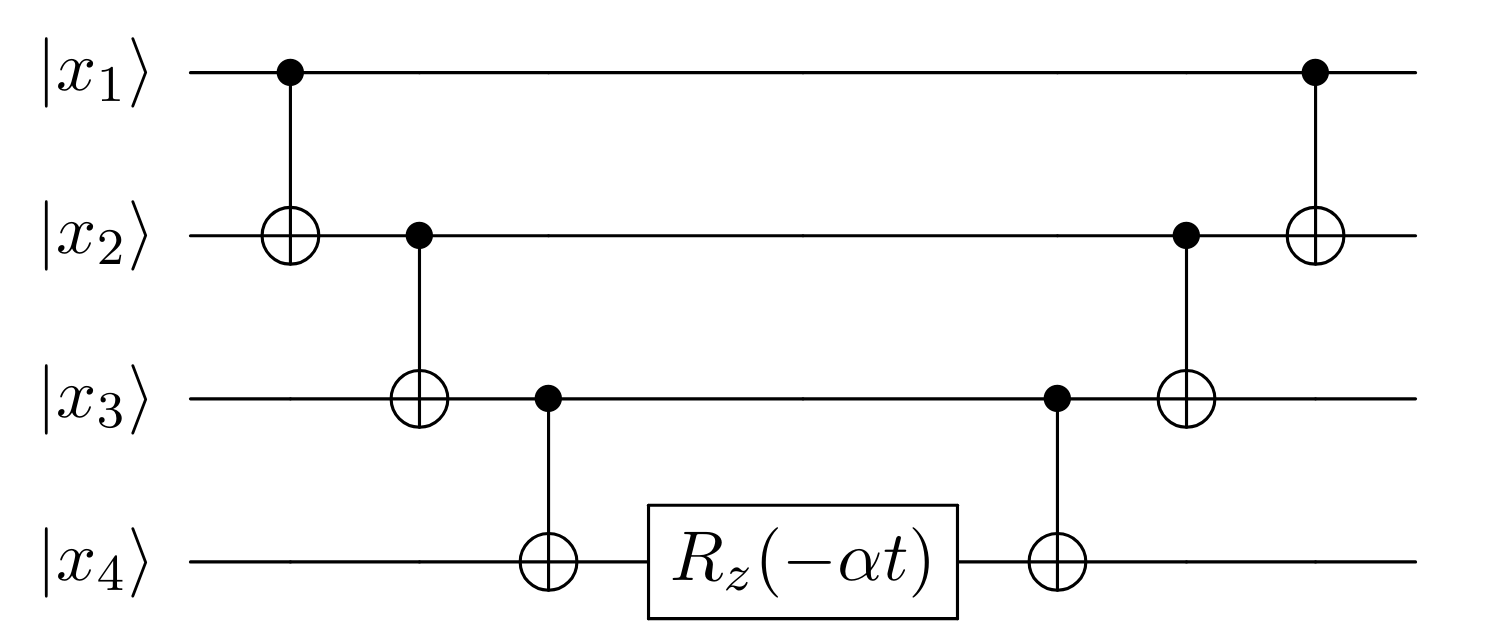
\includegraphics[width=0.8\textwidth]{rsc/circuit.png}
    \end{figure}

  \end{center}
  $R_z(\theta) = \begin{bmatrix} e^{i \theta} & 0 \\ 0 & e^{-i \theta} \end{bmatrix}$
\end{frame}

\begin{frame}{Generalization to Weighted Sums of Pauli Matrices}
  For $H$ as a weighted sum of commuting Pauli matrices:
  \begin{equation*}
    H = \sum_{j=1}^{m} \alpha_j \sigma_{s_j}
  \end{equation*}
  the evolution follows as:
  \begin{equation*}
    e^{-i H t} = \prod_{j=1}^{m} e^{-i \alpha_j \sigma_{s_j} t}
  \end{equation*}
  This requires $O(mn)$ quantum gates.
\end{frame}


%%%%%%%%%%%%%%%%%%% 
% Inigo
%%%%%%%%%%%%%%%%%%%



\begin{frame}{Non-Commuting Hamiltonians}
If \(A\) and \(B\) are non-commuting operators, we might have that
\[
e^{-i(A+B)t} \neq e^{-iAt}\,e^{-iBt}\,.
\]
In this case we can combine approximate simulations of
\(
e^{-iHt/p} 
\)
for some large \(p\). We will need two lemmas:
\begin{itemize}
    \item Error in approximate simulation concatenation.
    \item Lie-Trotter product formula.
\end{itemize}
\end{frame}

\begin{frame}{Lemma 1}
Let \((U_i){i=1}^m\) and \((V_i){i=1}^m\) be sequences of unitary operators satisfying
\[
\|U_i - V_i\| \le \epsilon \quad \text{for all } 1 \le i \le m.
\]
Then,
\[
\|U_m U_{m-1} \cdots U_1 - V_m V_{m-1} \cdots V_1\| \le m\,\epsilon.
\]

\textbf{Proof by induction:}

\begin{itemize}
  \item Base case: For \(m=1\), the claim is trivial.
  \item Inductive step: Assume the claim holds for \(m\). We need to show that
\(
\|U_{m+1}U_m \cdots U_1 - V_{m+1}V_m \cdots V_1\| \le (m+1)\epsilon.
\)
\end{itemize}

\end{frame}

\begin{frame}{Inductive step}
\[
\begin{aligned}
\|U_{m+1}U_m\cdots U_1 - V_{m+1}V_m\cdots V_1\| 
&= \\
\|U_{m+1}U_m\cdots U_1 \alert{-U_{m+1}V_m\cdots V_1} \\ \alert{+ U_{m+1}V_m\cdots V_1} 
- V_{m+1}V_m\cdots V_1\|
\pause
&\leq \\ 
\|U_{m+1}U_m\cdots U_1 \alert{-U_{m+1}V_m\cdots V_1}\| \\ + \|\alert{ U_{m+1}V_m\cdots V_1} 
- V_{m+1}V_m\cdots V_1\| 
\pause
&= \\
\|U_{m+1} (U_m\cdots U_1 -V_m\cdots V_1)\| \\ + \| V_m\cdots V_1
(U_{m+1} - V_{m+1})\|
\pause
&= \\
\cancel{\|U_{m+1}\|} \|(U_m\cdots U_1 -V_m\cdots V_1)\| \\ + \cancel{\|V_m\cdots V_1\|}\|
(U_{m+1} - V_{m+1})\|
\pause
&\leq \\
m\,\epsilon + \epsilon
\end{aligned}
\]
\end{frame}

\begin{frame}{Simulation technique}
Thus, in order to approximate 
\[
\prod_{j=1}^m e^{-iH_j t}
\]
to within \(\epsilon\), it suffices to approximate 
\[
e^{-iH_j t}
\]
for each \(j\) to within \(\epsilon/m\). 

\vspace{1em}
Next we show how this allows a sum of the form 
\[
e^{-i\left(\sum_{j} H_j\right)t}
\]
to be approximated.
\end{frame}

\begin{frame}{Lemma 2}
\textbf{Lie-Trotter product formula} \\
Let \(A\) and \(B\) be Hermitian matrices satisfying
\[
\|A\| \le \delta, \quad \|B\| \le \delta, \quad \text{with } \delta \le 1.
\]
Then,
\[
e^{-iA} e^{-iB} = e^{-i(A+B)} + O(\delta^2).
\]
Notation: \( E = O(\epsilon) \text{ means that the matrix satisfies }
\|E\| \le C\,\epsilon
\) for some universal constant $C$.

\end{frame}

\begin{frame}{Proof of Lemma 2}
\[
\begin{aligned}
e^{-iA} = I - iA + \sum_{k=2}^{\infty} \frac{(-iA)^k}{k!}
\pause
&= \\ I - iA + (-iA)^2 \sum_{k=0}^{\infty} \frac{(-iA)^k}{(k+2)!}
\pause
&= \\ I - iA + O(\|(-iA)^2\|) O(\|\sum_{k=0}^{\infty} \frac{(-iA)^k}{(k+2)!}\|)
\pause
&= \\ I - iA + O(\delta^2) O(\sum_{k=0}^{\infty} \frac{\delta^k}{(k+2)!})
\pause
&= \\ I - iA + O(\delta^2) \cancel{O(e^{\delta}})
\end{aligned}
\]
\pause
\[
e^{-iA} e^{-iB}
= \bigl(I - iA + O(\delta^2)\bigr)\bigl(I - iB + O(\delta^2)\bigr)
= I - iA - iB + O(\delta^2)
= e^{-i(A+B)} + O(\delta^2)
\]
\end{frame}

%%%%%%%%%%%%%%%%%%%
% Gonzalo
%%%%%%%%%%%%%%%%%%%

\begin{frame}{Hamiltonian Simulation Approximation}
We show how approximating a product of the form \(\prod_{j} e^{-iH_j t}\) allows a sum of the form \(e^{-i(\sum_{j} H_j )t}\) to be approximated.\newline\pause

We can now apply \textbf{Lemma 2} formula multiple times, for any Hermitian matrices \( H_1, \dots, H_m \) satisfying \( \|H_j\| \leq \delta \leq 1 \) for all \( j \) as follows,\pause
\begin{align*}
e^{-iH_1} e^{-iH_2} \dots e^{-iH_m} &= 
\left( e^{-i(H_1+H_2)} + O(\delta^2) \right) e^{-iH_3} \dots e^{-iH_m} \\  
&= \left( e^{-i(H_1+H_2+H_3)} + O((2\delta)^2) \right) e^{-iH_4} \dots e^{-iH_m} + O(\delta^2) \\  
&= e^{-i(H_1+\dots+H_m)} + O(\delta^2) + O((2\delta)^2) + \dots + O(((m-1)\delta)^2) \\  
&= e^{-i(H_1+\dots+H_m)} + O(m^3\delta^2)
\end{align*}
\end{frame}

\begin{frame}
    \frametitle{Hamiltonian Simulation Approximation}

    Write \( H = \sum_{j=1}^{m} H_j \), where \( \|H_j\| \leq \Delta \).  
    Applying this claim to matrices \( H_j t/p \) for any \( t \) and \( p \geq t \Delta \), we have: \pause
    
    \[
    \left\| e^{-iH_1 t/p} e^{-iH_2 t/p} \dots e^{-iH_m t/p} - e^{-i(H_1+\dots+H_m)t/p} \right\| = O \left( m^3 \left( \frac{t\Delta}{p} \right)^2 \right).
    \]\pause

    As an example, $H_j$ could be a weighted Pauli matrix as in the previous section, where the constraint corresponds to $|\alpha_j| \leq \Delta$.

\end{frame}

\begin{frame}
    \frametitle{Universal Constant and Approximation Bound}

    There exists a universal constant \( C \) such that for \( p \geq Cm^3 (t \Delta)^2 / \epsilon \): \pause

    \[
    \left\| e^{-iH_1 t/p} e^{-iH_2 t/p} \dots e^{-iH_m t/p} - e^{-i(H_1+\dots+H_m)t/p} \right\| \leq \frac{\epsilon}{p}.
    \]\pause

    By \textbf{Lemma 1}, for any such \( p \),\pause

    \[
    \left\| \left( e^{-iH_1 t/p} e^{-iH_2 t/p} \dots e^{-iH_m t/p} \right)^p - e^{-i(H_1+\dots+H_m)t} \right\| \leq \epsilon.
    \]\pause

    By this result, we can simulate a Hamiltonian for time \textit{t} by simulating the evolution of each of this terms for time $t/p$ and concatenating each of the simulations.

\end{frame}

\begin{frame}
    \frametitle{Hamiltonian Simulation Theorem}

    \begin{alertblock}{Theorem}
         Let \( H \) be a Hamiltonian written as:

        \[
        H = \sum_{S \in \{I, X, Y, Z\}^n} \alpha_S \sigma_S,
        \]
    
        where at most \( m \) coefficients \( \alpha_S \) are nonzero, and \( \max_S |\alpha_S| = O(1) \).  
        Then, for any \( t \), there exists a quantum circuit that approximates \( e^{-iHt} \) within \( \epsilon \) in time:
    
        \[
        O(m^4 n t^2 / \epsilon).
        \]
    
    \end{alertblock}

\end{frame}

\begin{frame}
    \frametitle{Computational Complexity Considerations}

    It seems undesirable that simulating a Hamiltonian for time \( t \) depends on \( t \) as \( O(t^2) \).  
    However, using more advanced techniques, this dependence can be improved to linear, up to logarithmic factors.

\end{frame}

\begin{frame}
    \frametitle{Recap}
Key points we have followed in order to showcase Hamiltonian simulation:
    \begin{itemize}
    
        \item Defined a notion of simulation
        \item Defined the circuit to simulate a Hamiltonian proportional to a Pauli matrix. $O(n)$
        \item Extend this result to the case in which the Hamiltonian is a sum of \textit{m} weighted Pauli matrices that commute. $O(nm)$
        \item Finally, see how to approximate the non commuting case.
    \end{itemize}

\end{frame}



\end{document}

%%% Local Variables:
%%% mode: LaTeX
%%% TeX-master: t
%%% End:
